\ifx\wholebook\relax \else
% ------------------------

\documentclass[UTF8]{article}
%------------------- Other types of document example ------------------------
%
%\documentclass[twocolumn]{IEEEtran-new}
%\documentclass[12pt,twoside,draft]{IEEEtran}
%\documentstyle[9pt,twocolumn,technote,twoside]{IEEEtran}
%
%-----------------------------------------------------------------------------
%
% loading packages
%

\RequirePackage{ifpdf}
\RequirePackage{ifxetex}

%
%
\ifpdf
  \RequirePackage[pdftex,%
       bookmarksnumbered,%
              colorlinks,%
          linkcolor=blue,%
              hyperindex,%
        plainpages=false,%
       pdfstartview=FitH]{hyperref}
\else\ifxetex
  \RequirePackage[bookmarksnumbered,%
               colorlinks,%
           linkcolor=blue,%
               hyperindex,%
         plainpages=false,%
        pdfstartview=FitH]{hyperref}
\else
  \RequirePackage[dvipdfm,%
        bookmarksnumbered,%
               colorlinks,%
           linkcolor=blue,%
               hyperindex,%
         plainpages=false,%
        pdfstartview=FitH]{hyperref}
\fi\fi
%\usepackage{hyperref}

% other packages
%--------------------------------------------------------------------------
\usepackage{graphicx, color}
\usepackage{subfig}
\usepackage{tikz}
\usetikzlibrary{matrix,positioning}

\usepackage{amsmath, amsthm, amssymb} % for math
\usepackage{exercise} % for exercise
\usepackage{import} % for nested input

%
% for programming
%
\usepackage{verbatim}
\usepackage{listings}
%\usepackage{algorithmic} %old version; we can use algorithmicx instead
\usepackage{algorithm}
\usepackage[noend]{algpseudocode} %for pseudo code, include algorithmicsx automatically
\usepackage{appendix}
\usepackage{makeidx} % for index support
\usepackage{titlesec}

\usepackage[cm-default]{fontspec}
\usepackage{xunicode}

% detect and select Chinese font
% ------------------------------
% the following cmd can list all availabe Chinese fonts in host.
% fc-list :lang=zh
\def\myfont{STHeiti}  % Under Mac OS X
\def\linuxfallback{WenQuanYi Micro Hei} % Under Linux
\def\winfallback{SimSun} % Under Windows
\suppressfontnotfounderror1 % Avoid setting exit code (error level) to break make process
\count255=\interactionmode
\batchmode
\font\foo="\myfont"\space at 10pt
\ifx\foo\nullfont
  \font\foo = "\linuxfallback"\space at 10pt
  \ifx\foo\nullfont
    \font\foo = "\winfallback"\space at 10pt
    \ifx\foo\nullfont
      \errorstopmode
      \errmessage{no suitable Chinese font found}
    \else
      \let\myfont=\winfallback % Windows
    \fi
  \else
    \let\myfont=\linuxfallback % Linux
  \fi
\fi
\interactionmode=\count255
\setmainfont[Mapping=tex-text]{\myfont}

\XeTeXlinebreaklocale "zh"  % to solve the line breaking issue
\XeTeXlinebreakskip = 0pt plus 1pt minus 0.1pt

\titleformat{\paragraph}
{\normalfont\normalsize\bfseries}{\theparagraph}{1em}{}
\titlespacing*{\paragraph}
{0pt}{3.25ex plus 1ex minus .2ex}{1.5ex plus .2ex}

\lstdefinelanguage{Smalltalk}{
  morekeywords={self,super,true,false,nil,thisContext}, % This is overkill
  morestring=[d]',
  morecomment=[s]{"}{"},
  alsoletter={\#:},
  escapechar={!},
  literate=
    {BANG}{!}1
    {UNDERSCORE}{\_}1
    {\\st}{Smalltalk}9 % convenience -- in case \st occurs in code
    % {'}{{\textquotesingle}}1 % replaced by upquote=true in \lstset
    {_}{{$\leftarrow$}}1
    {>>>}{{\sep}}1
    {^}{{$\uparrow$}}1
    {~}{{$\sim$}}1
    {-}{{\sf -\hspace{-0.13em}-}}1  % the goal is to make - the same width as +
    %{+}{\raisebox{0.08ex}{+}}1		% and to raise + off the baseline to match -
    {-->}{{\quad$\longrightarrow$\quad}}3
	, % Don't forget the comma at the end!
  tabsize=2
}[keywords,comments,strings]

% for better Haskell code outlook
\lstdefinelanguage{Haskell}{
  basicstyle=\small\ttfamily,
  flexiblecolumns=false,
  basewidth={0.5em,0.45em},
  literate={+}{{$+$}}1 {/}{{$/$}}1 {*}{{$*$}}1 {=}{{$=$}}1
           {>}{{$>$}}1 {<}{{$<$}}1 {\\}{{$\lambda$}}1
           {\\\\}{{\char`\\\char`\\}}1
           {->}{{$\rightarrow$}}2 {>=}{{$\geq$}}2 {<-}{{$\leftarrow$}}2
           {<=}{{$\leq$}}2 {=>}{{$\Rightarrow$}}2
           {\ .}{{$\circ$}}2 {\ .\ }{{$\circ$}}2
           {>>}{{>>}}2 {>>=}{{>>=}}2
           {|}{{$\mid$}}1
}[keywords,comments,strings]

\lstloadlanguages{C, C++, Lisp, Haskell, Python, Smalltalk}

\lstset{
  showstringspaces = false
}

% ======================================================================

\def\BibTeX{{\rm B\kern-.05em{\sc i\kern-.025em b}\kern-.08em
    T\kern-.1667em\lower.7ex\hbox{E}\kern-.125emX}}

%
% mathematics
%
\newcommand{\be}{\begin{equation}}
\newcommand{\ee}{\end{equation}}
\newcommand{\bmat}[1]{\left( \begin{array}{#1} }
\newcommand{\emat}{\end{array} \right) }
\newcommand{\VEC}[1]{\mbox{\boldmath $#1$}}

% numbered equation array
\newcommand{\bea}{\begin{eqnarray}}
\newcommand{\eea}{\end{eqnarray}}

% equation array not numbered
\newcommand{\bean}{\begin{eqnarray*}}
\newcommand{\eean}{\end{eqnarray*}}

\newtheorem{theorem}{Theorem}[section]
\newtheorem{lemma}[theorem]{Lemma}
\newtheorem{proposition}[theorem]{Proposition}
\newtheorem{corollary}[theorem]{Corollary}


\setcounter{page}{1}

\begin{document}

%--------------------------

% ================================================================
%                 COVER PAGE
% ================================================================

\title{Radix树-Trie和Patricia}

\author{Larry~LIU~Xinyu
\thanks{{\bfseries Larry LIU Xinyu } \newline
  Email: liuxinyu95@gmail.com \newline}
  }

\maketitle
\fi

\markboth{Radix树-Trie和Patricia}{初等算法}

\ifx\wholebook\relax
\chapter{Radix树-Trie和Patricia}
\numberwithin{Exercise}{chapter}
\fi

%{\bfseries Corresponding Author:} Larry LIU Xinyu


% ================================================================
%                 Introduction
% ================================================================
\section{简介}
\label{introduction}
\index{Radix tree}

前面章节介绍的二叉树都是利用节点来存储信息,我们也可以利用边(edge)来存储。Radix树(中文亦译作基数树),如Trie和Patricia就是这样的数据结构。它们产生于1960年代,被广泛用于编译器\cite{okasaki-int-map}和生物信息处理(如DNA模式匹配)\cite{wiki-suffix-tree}等领域。

\begin{figure}[htbp]
  \centering
  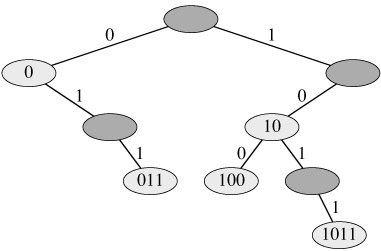
\includegraphics[scale=0.4]{img/radix-tree.ps}
  \caption{Radix树} \label{fig:radix-tree}
\end{figure}

图\ref{fig:radix-tree}展示了一棵radix树\cite{CLRS}。它包含了串1011、10、011、100和0。如果要在其中查找$k=(b_0b_1...b_n)_2$,我们首先检查$b_0$(左侧的MSB)是1还是0,如果为0,我们接下来去左侧分支查找;如果为1,则去右侧分支查找。然后,我们检查第二位,并重复这一过程直到处理完所有的n位或者遇到了一个叶子节点。

Radix树并不在节点中存储key,信息由边来代表。图中节点中标注的key仅仅是为了方便理解。

人们自然要问:“可以用整数取代串来代表key么?”由于整数可以用二进制来表示,因此这样可以节省空间,而且使用位运算后,速度也可以加快。

% ================================================================
%                 Int Trie
% ================================================================
\section{整数Trie}
\label{int-trie}
\index{Radix tree!整数trie}

图\ref{fig:radix-tree}中所示的数据结构常被称为\emph{binary trie}。Trie是Edward Fredkin提出的。它来自英文单词retrieval,最开始发音为/'tri:/。但是许多人都把它读作/'trai/(和英文单词try的发音相同)\cite{wiki-trie}。Trie也被成为前餟树(prefix tree)。一棵binary trie是一种特殊的二叉树,每个key存放的位置由它的二进制各个位来决定。每个0表示“向左”,而1表示“向右”\cite{okasaki-int-map}。

由于整数可以表示位二进制,我们可以直接使用整数来代替0/1串作为key。当把一个整数插入到trie时,我们首先将其转化为二进制,然后检查第一位,若为0,则递归插入左侧分支,否则若为1则插入右侧分支。

但是这里右一个问题,考虑图\ref{fig:big-endian-trie}中的trie。如果使用0/1串,这3个key是各不相同的。但它们却代表同一个十进制整数。就这个例子来说,我们应该在trie中的哪个位置插入整数3呢?

\begin{figure}[htbp]
  \centering
  \includegraphics[scale=0.4]{img/big-endian-trie.ps}
  \caption{大端(big-endian)trie} \label{fig:big-endian-trie}
\end{figure}

一个办法是将所有有效位前的0也当作有效位。如果整数由32位表示,我们向一个空trie插入1,结果将是一个有32层分支的树。其中的31个中间节点只有一个左子树,最后一个节点只有一个右子树。空间利用率很低。

Okasaki给出了一种解决方法\cite{okasaki-int-map}。我们通常把二进制的高位(MSB)放在左边,低位(LSB)放在右边。这样的trie称作大端(big-endian)树。相反,我们可以使用小端(little-endian)来表示key。这样,十进制的1表示为小端二进制的1。如果插入到空trie中,结果就是含有一个右侧叶子节点的根。只有一层分支。十进制的2将被表示为小端二进制的01,十进制的3表示为小端二进制$(11)_2$。这样就消除了有效位前面的0,每一个整数key在trie中的位置可以被唯一确定。

%=========================================================================
%       Definition of integer trie
%=========================================================================
\subsection{整数Trie的定义}
我们可以复用二叉树的结构来定义binary trie。一个binary trie的节点要么为空,要么包含左右两个分支。非空节点也可以保存额外的数据,称为卫星数据(satellite data)。左侧分支编码为0,右侧分支编码为1。

下面的Haskell例子代码定义了trie的代数数据类型(algebraic data type)。

\lstset{language=Haskell}
\begin{lstlisting}
data IntTrie a = Empty
               | Branch (IntTrie a) (Maybe a) (IntTrie a)
\end{lstlisting}

在命令式编程语言中,Trie通常被定义为结构,如下面的Python例子代码所示:

\lstset{language=Python}
\begin{lstlisting}
class IntTrie:
    def __init__(self):
        self.left = self.right = None
        self.value = None
\end{lstlisting}


% ================================================================
%               Insertion of integer trie
% ================================================================
\subsection{插入}
\index{整数trie!插入}

由于key是小端整数,插入时,我们需要从右侧逐位进行处理。如果为0,则递归插入左子树,否则为1,需要插入右子树。如果子树为空,我们需要创建一个新节点。重复这一步骤直到处理完最后一位(最左侧的位)后停止。

%\begin{algorithm}
\begin{algorithmic}[1]
\Function{Insert}{$T, k, v$}
  \If{$T =$ NIL}
    \State $T \gets$ \Call{Empty-Node}{}
  \EndIf
  \State $p \gets T$
  \While{$k \neq 0$}
    \If{\Call{Even?}{$k$}}
      \If{\Call{Left}{$p$} = NIL}
        \State \Call{Left}{$p$} $\gets$ \Call{Empty-Node}{}
      \EndIf
      \State $p \gets$ \Call{Left}{$p$}
    \Else
      \If{\Call{Right}{$p$} = NIL}
        \State \Call{Right}{$p$} $\gets$ \Call{Empty-Node}{}
      \EndIf
      \State $p \gets$ \Call{Right}{$p$}
    \EndIf
    \State $k \gets \lfloor k/2 \rfloor$
  \EndWhile
  \State \Call{Data}{$p$} $\gets v$
  \State \Return $T$
\EndFunction
\end{algorithmic}
%\end{algorithm}

插入算法接受3个参数:一棵trie树$T$、一个key $k$和相应的数据$v$。下面的Python例子程序实现了这一算法。可以没有额外的数据,它缺省为空。

\lstset{language=Python}
\begin{lstlisting}
def trie_insert(t, key, value = None):
    if t is None:
        t = IntTrie()
    p = t
    while key != 0:
        if key & 1 == 0:
            if p.left is None:
                p.left = IntTrie()
            p = p.left
        else:
            if p.right is None:
                p.right = IntTrie()
            p = p.right
        key = key>>1
    p.value = value
    return t
\end{lstlisting}

图\ref{int-trie}的例子是向一棵空trie中插入key和value对\{$ 1 \rightarrow a, 4 \rightarrow b, 5 \rightarrow c, 9 \rightarrow d$\}的结果。

\begin{figure}[htbp]
  \centering
  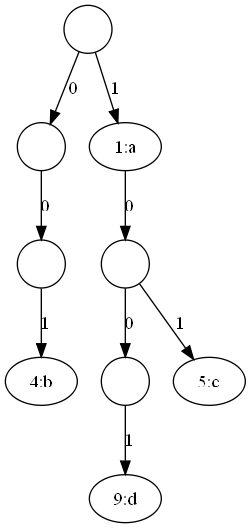
\includegraphics[scale=0.5]{img/int-trie.ps}
  \caption{用小端(little-endian)整数binary trie实现的映射(map):
          \{$ 1 \rightarrow a, 4 \rightarrow b, 5 \rightarrow c, 9 \rightarrow d$\}。}
  \label{fig:int-trie}
\end{figure}

由于整数trie的定义本身是递归的,插入算法可以很自然地用递归进行定义。如果最左侧的位为0,说明待插入的key为偶数,我们解下来递归在左侧分支进行插入;否则若最左侧的位为1,说明key为奇数,我们转向右侧分支。我们不断将key除以2并取整以取掉最左侧的位,直到处理完所有的位。此时key变为0,插入结束。记trie $T$的左右分支为$T_l$和$T_r$,节点上纯储的数据待为$d$(可以为空)。如果$T$为空,则其左右分支和数据也定义为空。我们可以这样定义插入算法:

\be
insert(T, k, v) = \left \{
  \begin{array}
  {r@{\quad:\quad}l}
  (T_l, v, T_r) & k = 0 \\
  (insert(T_l, k / 2, v), d, T_r) & even(k) \\
  (T_l, d, insert(T_r, \lfloor k / 2 \rfloor, v)) & otherwise
  \end{array}
\right.
\ee

如果待插入的key已经存在,这一算法会覆盖原来纯储的数据。也可以采用其他处理方法,如使用链表保存新数据而不是覆盖。

下面的Haskell例子程序实现了这一插入算法。

\lstset{language=Haskell}
\begin{lstlisting}
insert t 0 x = Branch (left t) (Just x) (right t)
insert t k x | even k = Branch (insert (left t) (k `div` 2) x) (value t) (right t)
             | otherwise = Branch (left t) (value t) (insert (right t) (k `div` 2) x)

left (Branch l _ _) = l
left Empty = Empty

right (Branch _ _ r) = r
right Empty = Empty

value (Branch _ v _) = v
value Empty = Nothing
\end{lstlisting}

对于有$m$二进制位的整数$k$,这一算法递归$m$次,因此时间复杂度为$O(m)$。

% ================================================================
%               Look up in integer binary trie
% ================================================================
\subsection{查找}
\index{整数trie!查找}

在整数binary trie中查找key $k$时,我们从$k$的右侧,逐位检查,如果为0,就继续在左侧分支查找,否则若为1,则在右侧分支查找。当所有位都处理完,查找结束。

\begin{algorithmic}[1]
\Function{Lookup}{$T, k$}
  \While{$x \neq 0 \land T \neq $NIL}
    \If{ \Call{Even?}{$x$} }
      \State $T \gets$ \Call{Left}{$T$}
    \Else
      \State $T \gets$ \Call{Right}{$T$}
    \EndIf
    \State $k \gets \lfloor k/2 \rfloor$
  \EndWhile
  \If{$T \neq $ NIL}
    \State \Return \Call{Data}{$T$}
  \Else
    \State \Return not found \EndIf
\EndFunction
\end{algorithmic}

下面的Python例子程序使用了位操作来实现查找算法。

\lstset{language=Python}
\begin{lstlisting}
def lookup(t, key):
    while key != 0 and (t is not None):
        if key & 1 == 0:
            t = t.left
        else:
            t = t.right
        key = key>>1
    if t is not None:
        return t.value
    else:
        return None
\end{lstlisting}

查找操作也可以递归定义。如果树为空,则查找失败;如果$k=0$,则返回当前根节点中存储的数据。否则根据最后一位是0还是1,递归在左右分支进行查找。

\be
lookup(T, k) =  \left \{
  \begin{array}
  {r@{\quad:\quad}l}
  \phi & T = \phi \\
  d & k = 0 \\
  lookup(T_l, k / 2) & even(k) \\
  lookup(T_r, \lfloor k / 2 \rfloor) & otherwise
  \end{array}
\right.
\ee

下面的Haskell例子程序实现了递归查找算法。

\lstset{language=Haskell}
\begin{lstlisting}
search Empty k = Nothing
search t 0 = value t
search t k = if even k then search (left t) (k `div` 2)
             else search (right t) (k `div` 2)
\end{lstlisting}

若待查找的key有$m$位,则查找算法的复杂度为$O(m)$。

% ================================================================
%               Int Patricia
% ================================================================
\section{整数Patricia}
\label{int-patricia}
\index{整数Patricia}
\index{整数前餟树}

Trie最大的缺点是浪费空间。如图\ref{int-trie}所示,只有叶子节点存储了最终的数据。大多数情况下,整数trie中存在许多只包含一个孩子的节点。为了提高空间利用率,我们可以将一连串“独生子女”压缩成一个节点。Patricia就是这样的数据结构,由Donald R. Morrison在1968年提出。Patricia是英文:Practical algorithm to retrieve information coded in alphanumeric的首字母缩写\cite{patricia-morrison}。它本质上是一种前餟树。

Okasaki给出了整数Patricia的实现\cite{okasaki-int-map}。将图\ref{fig:int-trie}中只有一个子树的节点合并为后,可以得到一棵如图\ref{fig:little-endian-patricia}所示的树。

\begin{figure}[htbp]
  \centering
  \includegraphics[scale=0.5]{img/little-endian-patricia.ps}
  \caption{小端(Little endian)Patricia实现的映射
     \{$ 1 \rightarrow a, 4 \rightarrow b, 5 \rightarrow c, 9 \rightarrow d$\}。}
  \label{fig:little-endian-patricia}
\end{figure}

观察此图,可以发现分支节点所代表的key是它包含的所有分支的公共前餟。这些分支的key一开始都一样,然后从某一点开始出现不同。和trie相比,Patricia节省了很多空间。

和整数trie不同,Patricia可以使用大端(big-endian)而不会遇到\ref{int-trie}中所描述的0前餟问题。第一位有效数字前的0全都被去除以节省空间。Okasaki在\cite{okasaki-int-map}中列出了大端patricia的优点。

% ================================================================
%                 Definition of int patricia tree
% ================================================================
\subsection{定义}

整数patricia是一种特殊的二叉树。它或者为空,或者是一个节点。节点有两种类型:

\begin{itemize}
\item 叶子节点:包含一个整数key和相应的数据(可以没有数据);
\item 分支节点:包含左右子分支。两个子分支的key具有最长的二进制公共前缀。其中左左侧子分支的下一位是0,而右侧子分支的下一位是1。
\end{itemize}

下面的Haskell例子代码定义了patricia:

\lstset{language=Haskell}
\begin{lstlisting}
type Key = Int
type Prefix = Int
type Mask = Int

data IntTree a = Empty
               | Leaf Key a
               | Branch Prefix Mask (IntTree a) (IntTree a)
\end{lstlisting}

为了表示从哪一位开始左右分支的key变得不相同,分支节点中保存了mask(掩码)信息。通常mask是2的整数次幂,形如$2^n$其中$n$是非负整数。所有低于$n$的二进制位都不属于key的公共前缀。

下面的Python例子代码定义了patricia和相应的辅助函数。

\lstset{language=Python}
\begin{lstlisting}
class IntTree:
    def __init__(self, key = None, value = None):
        self.key = key
        self.value = value
        self.prefix = self.mask = None
        self.left = self.right = None

    def set_children(self, l, r):
        self.left = l
        self.right = r

    def replace_child(self, x, y):
        if self.left == x:
            self.left = y
        else:
            self.right = y

    def is_leaf(self):
        return self.left is None and self.right is None

    def get_prefix(self):
        if self.prefix is None:
            return self.key
        else:
            return self.prefix
\end{lstlisting}


% ================================================================
%                 Insertion of int patricia tree
% ================================================================
\subsection{插入}
\index{整数patricia!插入}
当插入key时,如果树为空,结果为一个叶子节点,key和相关的数据存储于节点中,如图\ref{fig:int-patricia-insert-a}所示。

\begin{figure}[htbp]
  \centering
    \begin{tikzpicture}[scale=1,
      treenode/.style={circle, draw, inner sep= 0pt, minimum size = .6cm}]
    \node[treenode] at (-2, 0) {NIL};
    \node[treenode] at (2, 0) {12};
    \end{tikzpicture}
  %\includegraphics[scale=0.8]{img/int-patricia-insert-a.ps}
  \caption{左侧:树为空;右侧:插入key12后。}
  \label{fig:int-patricia-insert-a}
\end{figure}

如果树只有一个叶子节点$x$,我们把待插入的key和数据放入一个新的叶子节点$y$中。然后创建一个新的分支节点,并令$x$和$y$为这一新分支节点的两个子节点。为了确定$y$应该在左边还是右边,我们需要找到$x$和$y$的最长公共前餟。举个例子,假设$key(x)$为12(二进制1100),$key(y)$为15(二进制1111),则最长公共前餟为二进制$11oo$,其中$o$代表的二进制位我们并不关心,我们可以使用一个整数来mask掉这些不关心的位。在这个例子中,可以用4(二进制100)作为mask。最长公共前餟后面的一位代表$2^1$。$key(x)$中这一位是0,而$key(y)$中这一位是1。因此$x$是左子树,而$y$是右子树。这个例子如图\ref{fig:int-patricia-insert-b}所示。

\begin{figure}[htbp]
  \centering
  \includegraphics[scale=0.7]{img/int-patricia-insert-b.ps}
  \caption{左侧:只含有一个叶子节点12的树;右侧:插入key 15后。}
  \label{fig:int-patricia-insert-b}
\end{figure}

如果树既不为空,也不是一个单独的叶子节点,我们需要先比较待插入的key和根节点中纪录的最长公共前餟是否一致。如果一致,则根据接下来的位是0还是1决定在左侧还是右侧递归进行插入。例如,若将整数14(二进制1110)插入图\ref{fig:int-patricia-insert-b}中所示的树中,由于最长公共前餟是$11oo$而接下来的一位($2^1$位)是1,所以需要将14递归插入到右子树。

最后,如果待插入的key和根节点中纪录的最长公共前餟不一致,我们需要从根节点分出一个新的枝杈。图\ref{fig:int-patricia-insert-c}展示了这两种不同的情况。

\begin{figure}[htbp]
  \centering
  \subfloat[插入key 14。它和最长公共前餟$(1100)_2$一致。需要将其递归插入到右侧分支中。]{\includegraphics[scale=0.5]{img/int-patricia-insert-c.ps}}\\
  \subfloat[插入key 5。它和最长公共前餟$(1100)_2$不一致。需要新分杈出一个分支。]{\includegraphics[scale=0.5]{img/int-patricia-insert-d.ps}}
  \caption{向分支节点插入key。}
  \label{fig:int-patricia-insert-c}
\end{figure}

记key为$k$,数据为$v$的节点为$(k, v)$,分支节点记为$(p, m, T_l, T_r)$,其中$p$代表最长公共前餟,$m$表示mask,$T_l$和$T_r$分别代表左右子分支。上述情况可以归纳为下面的插入算法:

\be
insert(T, k, v) = \left \{
  \begin{array}
  {r@{\quad:\quad}l}
  (k, v) & T = \phi \lor T = (k, v') \\
  join(k, (k, v), k', T) & T = (k', v') \\
  (p, m, insert(T_l, k, v), T_r) & T = (p, m, T_l, T_r), match(k, p, m), zero(k, m) \\
  (p, m, T_l, insert(T_r, k, v)) & T = (p, m, T_l, T_r), match(k, p, m), \lnot zero(k, m) \\
  join(k, (k, v), p, T) & T = (p, m, T_l, T_r), \lnot match(k, p, m)
  \end{array}
\right.
\ee

第一行处理边界情况,$T$或者为空,或者是一个表示同样key的叶子节点。这里我们用新的值覆盖以前存在的数据。

第二行处理$T$为叶子节点,但是key不同的情况。这时需要分支出一个新的叶子节点,为此,我们需要计算出最长公共前餟,并判断哪个在左侧,哪个在右侧。函数$join(k_1, T_1, K_2, T_2)$负责这些处理,我们稍后会定义它。

第三、四行处理$T$为分支节点,且分支代表的前餟和待插入的key一致的情况。如果接下来的一位是0,则第三行会递归向左侧分支进行插入。否则第四行递归向右侧分支插入。

最后一行处理$T$为分支节点,但是key不一致的情况。我门需要调用$join$函数来分支出一个新的叶子节点。

接下来需要定义函数$match(k, p, m)$用以判断整数$k$在掩码$m$以上的位是否和$p$一致。也就是检查$p$在掩码以上的位是否为$k$的一个前餟。例如,一个分支节点的key表示为二进制为$(p_np_{n-1} ... p_i...p_0)_2$,待插入的key $k$的二进制形式为$(k_nk_{n-1} ... k_i ... k_0)_2$,掩码mask为$(100...0)_2=2^i$。则称$k$、$p$、$m$一致当且仅当对于任意$j$, $i \leq j \leq n$有$p_j=k_j$。

我们可以通过判断等式$mask(k, m) = p$来实现$match$函数。其中$mask(x, m) = \overline{m-1} \& x$。即先对$m-1$按位取反,然后将结果和$x$按位进行与运算。

函数$zero(k, m)$检查公共前餟后接下来的一位是否为0。我们可以将掩码$m$向右做1位移位运算,接下来和$k$进行按位与运算。

\be
zero(k, m) = x \& shift_r(m, 1)
\ee

举例来说,若$m = (100..0)_2 = 2^i$、$k = (k_nk_{n-1}...k_i1...k_0)_2$,由于$k_i$的下一位是1,所以$zero(k, m)$的结果为false;反之,若$k = (k_nk_{n-1}...k_i0...k_0)_2$,则结果为true。

函数$join(p_1, T_1, p_2, T_2)$接受两个前餟和两棵树作为参数。它找出$p_1$与$p_2$的最长公共前餟,然后创建一个新的分支节点,并将$T_1$和$T_2$作为子节点。

\be
join(p_1, T_1, p_2, T_2) = \left \{
  \begin{array}
  {r@{\quad:\quad}l}
  (p, m, T_1, T_2) & zero(p1, m), (p, m) = LCP(p_1, p_2) \\
  (p, m, T_2, T_1) & \lnot zero(p1, m)
  \end{array}
\right.
\ee

为了计算$p_1$和$p_2$的最长公共前缀,我们可以先对它们计算异或(exclusive-or),然后用这个结果的有效位数产生一个掩码$m = 2^{|xor(p_1,p_2)|}$。最长公共前缀就可以用这个掩码和$p_1$与$p_2$中的任何一个得出。例如:

\be
p = mask(p_1, m)
\ee

下面的Haskell例子程序实现了插入算法:

\lstset{language=Haskell}
\begin{lstlisting}
import Data.Bits

insert t k x
   = case t of
       Empty -> Leaf k x
       Leaf k' x' -> if k==k' then Leaf k x
                     else join k (Leaf k x) k' t -- t@(Leaf k' x')
       Branch p m l r
          | match k p m -> if zero k m
                           then Branch p m (insert l k x) r
                           else Branch p m l (insert r k x)
          | otherwise -> join k (Leaf k x) p t -- t@(Branch p m l r)

join p1 t1 p2 t2 = if zero p1 m then Branch p m t1 t2
                                else Branch p m t2 t1
    where
      (p, m) = lcp p1 p2

lcp :: Prefix -> Prefix -> (Prefix, Mask)
lcp p1 p2 = (p, m) where
    m = bit (highestBit (p1 `xor` p2))
    p = mask p1 m

highestBit x = if x == 0 then 0 else 1 + highestBit (shiftR x 1)

mask x m = (x .&. complement (m-1)) -- complement means bit-wise not.

zero x m = x .&. (shiftR m 1) == 0

match k p m = (mask k m) == p
\end{lstlisting}

插入算法也可以用命令式(imperative)的方式实现:

\begin{algorithmic}[1]
\Function{Insert}{$T, k, v$}
  \If{$T = $ NIL}
    \State $T \gets$ \Call{Create-Leaf}{$k, v$}
    \State \Return $T$
  \EndIf
  \State $y \gets T$
  \State $p \gets$ NIL
  \While{$y$ is not leaf, and \textproc{Match}($k$, \Call{Prefix}{$y$}, \Call{Mask}{$y$})}
    \State $p \gets y$
    \If{\textproc{Zero?}($k$, \Call{Mask}{$y$})}
      \State $y \gets$ \Call{Left}{$y$}
    \Else
      \State $y \gets$ \Call{Right}{$y$}
    \EndIf
  \EndWhile
  \If{$y$ is leaf, and $k = $ \Call{Key}{$y$}}
    \State \Call{Data}{$y$} $\gets v$
  \Else
    \State $z \gets$ \textproc{Branch}($y$, \Call{Create-Leaf}{$k, v$})
    \If{$p = $ NIL}
      \State $T \gets z$
    \Else
      \If{\Call{Left}{$p$} $ = y$}
        \State \Call{Left}{$p$} $\gets z$
      \Else
        \State \Call{Right}{$p$} $\gets z$
      \EndIf
    \EndIf
  \EndIf
  \State \Return $T$
\EndFunction
\end{algorithmic}

函数\textproc{Branch}($T_1, T_2$)的作用和前面定义的$join$类似。它创建一个新的分支节点,计算最长公共前缀,然后将$T_1$和$T_2$设置为这一分支的两棵子树。

\begin{algorithmic}[1]
\Function{Branch}{$T_1, T_2$}
  \State $T \gets$ \Call{Empty-Node}{}
  \State $($ \Call{Prefix}{$T$}, \Call{Mask}{$T$} $) \gets$ \textproc{LCP}(\Call{Prefix}{$T_1$}, \Call{Prefix}{$T_2$})
  \If{\textproc{Zero?}(\Call{Prefix}{$T_1$}, \Call{Mask}{$T$})}
    \State \Call{Left}{$T$} $\gets T_1$
    \State \Call{Right}{$T$} $\gets T_2$
  \Else
    \State \Call{Left}{$T$} $\gets T_2$
    \State \Call{Right}{$T$} $\gets T_1$
  \EndIf
  \State \Return $T$
\EndFunction
\end{algorithmic}

下面的Python例子程序实现了插入算法:

\lstset{language=Python}
\begin{lstlisting}
def insert(t, key, value = None):
    if t is None:
        t = IntTree(key, value)
        return t

    node = t
    parent = None
    while(True):
        if match(key, node):
            parent = node
            if zero(key, node.mask):
                node = node.left
            else:
                node = node.right
        else:
            if node.is_leaf() and key == node.key:
                node.value = value
            else:
                new_node = branch(node, IntTree(key, value))
                if parent is None:
                    t = new_node
                else:
                    parent.replace_child(node, new_node)
            break
    return t
\end{lstlisting}

辅助函数\texttt{match}, \texttt{branch}, \texttt{lcp}等定义如下:

\begin{lstlisting}
def maskbit(x, mask):
    return x & (~(mask-1))

def match(key, tree):
    return (not tree.is_leaf()) and maskbit(key, tree.mask) == tree.prefix

def zero(x, mask):
    return x & (mask>>1) == 0

def lcp(p1, p2):
    diff = (p1 ^ p2)
    mask=1
    while(diff!=0):
        diff>>=1
        mask<<=1
    return (maskbit(p1, mask), mask)

def branch(t1, t2):
    t = IntTree()
    (t.prefix, t.mask) = lcp(t1.get_prefix(), t2.get_prefix())
    if zero(t1.get_prefix(), t.mask):
        t.set_children(t1, t2)
    else:
        t.set_children(t2, t1)
    return t
\end{lstlisting}

图\ref{fig:int-patricia-haskell-insert}展示了使用插入算法构造的Patricia树。

\begin{figure}[htbp]
  \centering
  \includegraphics[scale=0.6]{img/int-patricia-haskell-insert.ps}
  \caption{插入映射$1 \rightarrow x, 4 \rightarrow y, 5 \rightarrow z$到一个大端整数Patricia树后的结果。}
  \label{fig:int-patricia-haskell-insert}
\end{figure}


% ================================================================
%                 Lookup in int patricia tree
% ================================================================
\subsection{查找}
\index{整数Patricia!查找}

根据Patricia的性质,当我们查找一个key时,如果它和根节点有相同的前缀,我们需要检查前缀后的位。如果这一位是0,我们需要接下来在左子树查找;否则如果为1,我们需要在右子树继续查找。

当到达一个叶子节点时,我们需要比较节点的key是否等于待查找的key。算法描述如下:

\begin{algorithmic}[1]
\Function{Look-Up}{$T, k$}
  \If{$T =$ NIL}
    \State \Return $NIL$ \Comment{Not found}
  \EndIf
  \While{$T$ is not leaf, and \textproc{Match}($k$, \Call{Prefix}{$T$}, \Call{Mask}{$T$})}
    \If{\textproc{Zero?}($k$, \Call{Mask}{$T$})}
      \State $T \gets$ \Call{Left}{$T$}
    \Else
      \State $T \gets$ \Call{Right}{$T$}
    \EndIf
  \EndWhile
  \If{$T$ is leaf, and \Call{Key}{$T$} $=k$}
    \State \Return \Call{Data}{$T$}
  \Else
    \State \Return $NIL$ \Comment{Not found}
  \EndIf
\EndFunction
\end{algorithmic}

下面的Python例子程序实现了这一查找算法。

\lstset{language=Python}
\begin{lstlisting}
def lookup(t, key):
    if t is None:
        return None
    while (not t.is_leaf()) and match(key, t):
        if zero(key, t.mask):
            t = t.left
        else:
            t = t.right
    if t.is_leaf() and t.key == key:
        return t.value
    else:
        return None
\end{lstlisting}

查找算法也可以用递归的方式加以实现。如果Patricia树为空,或者它仅仅包含一个叶子节点,且节点的key不等于待查找的值,则查找失败,查找结果为空。如果待查找的树是一个叶子节点,且节点的key恰好等于待查找的值,则查找成功,查找结果就是该叶子节点所包含的数据。否则,如果树$T$是一个分支节点,我们需要比较节点存储的最长公共前缀是否和待查找的key一致,然后根据下一位是0还是1进行递归查找。如果最长公共前缀不一致,说明待查找的key不存在,我们返回空的查找结果表示查找失败。

\be
lookup(T, k) = \left \{
  \begin{array}
  {r@{\quad:\quad}l}
  \phi & T = \phi \lor (T = (k', v), k' \neq k) \\
  v & T = (k', v), k' = k \\
  lookup(T_l, k) & T = (p, m, T_l, T_r), match(k, p, m), zero(k, m) \\
  lookup(T_r, k) & T = (p, m, T_l, T_r), match(k, p, m), \lnot zero(k, m) \\
  \phi & otherwise
  \end{array}
\right.
\ee

下面的Haskell例子程序实现了递归查找算法。

\lstset{language=Haskell}
\begin{lstlisting}
search t k
  = case t of
      Empty -> Nothing
      Leaf k' x -> if k==k' then Just x else Nothing
      Branch p m l r
             | match k p m -> if zero k m then search l k
                              else search r k
             | otherwise -> Nothing
\end{lstlisting}


% ================================================================
%                 Alphabetic trie
% ================================================================
\section{字符Trie}
\index{Trie}

整数Trie和Patricia可以作为一个很好的起点。相关技术在编译器实现中有着重要的应用。Okasaki指出Haskell编译器GHC(Glasgow Haskell Compiler)在1998年以前,已经广泛使用了类似的实现\cite{okasaki-int-map}。

如果我们将key的类型扩展为字符,Trie和Patricia就可以称为解决文字处理相关的问题的有力武器。

% ================================================================
%                 Definition of Alphabetic trie
% ================================================================
\subsection{定义}
如果用字符作为key,仅仅使用左右两个分支就不够了。拿英语来说,一共有26个字符,每个字符还有大小写两种情况。如果忽略大小写,一种简单的办法是限定分支(子树)的个数不得超过26。有些简化的ANSI C实现使用长度为26的数组来管理分支。如图\ref{fig:trie-of-26}所示。

\begin{figure}[htbp]
  \centering
  \includegraphics[scale=0.45]{img/trie-of-26.ps}
  \caption{最多含有26个分支的字符Trie,包含'a'、'an'、'another'、'bool'、'boy'和'zoo'共6个key。}
  \label{fig:trie-of-26}
\end{figure}

并非所有的26个分支都含有数据。例如,图\ref{fig:trie-of-26}中,根节点的分支中,只有代表'a'、'b'和'z'的3个子分支不为空。其他分支,例如代表'c'的分支,全部是空的。简单起见,我们在接下来的部份,不画出这些空的分支。

如果区分大小写,或者处理英语以外的其他语言,分支的数目会超过26。我们可以通过使用Hash表或者map等数据结构来解决动态数目分支的情况。

综上,一棵字符trie或者为空,或者是一个节点。节点的类型有两种:

\begin{itemize}
\item 叶子节点,不含有任何子分支;
\item 分支节点,含有多个子分支,每个子分支都代表一个不同的字符。
\end{itemize}

叶子节点和分支节点都可能存储相关的数据(satellite data)。下面的Haskell例子代码定义了字符trie。

\lstset{language=Haskell}
\begin{lstlisting}
data Trie a = Trie { value :: Maybe a
                   , children :: [(Char, Trie a)]}

empty = Trie Nothing []
\end{lstlisting}

下面的ANSI C例子代码给出了字符trie的结构定义。简单起见,我们限定字符集仅仅包含小写英文字母'a'到'z'。

\lstset{language=C}
\begin{lstlisting}
struct Trie {
  struct Trie* children[26];
  void* data;
};
\end{lstlisting}


% ================================================================
%                 Insertion of Alphabetic trie
% ================================================================
\subsection{插入}
\index{Trie!插入}

插入一个字符串时,我们从根节点开始,逐一检查字符串中的每个字符和相应的分支。如果为空,就创建一个新的节点,然后处理下一个字符和对应的分支。我们重复这一过程直到处理完所有的字符。最后将数据存入此刻到达的节点。

插入算法的描述如下:

\begin{algorithmic}[1]
\Function{Insert}{$T, k, v$}
  \If{$T = $ NIL}
    \State $T \gets $ \Call{Empty-Node}{}
  \EndIf
  \State $p \gets T$
  \For{each $c$ in $k$}
    \If{\Call{Children}{$p$}[c] = NIL}
      \State \Call{Children}{$p$}[c] $\gets$ \Call{Empty-Node}{}
    \EndIf
    \State $p \gets $ \Call{Children}{$p$}[c]
  \EndFor
  \State \Call{Data}{$p$} $\gets v$
  \State \Return $T$
\EndFunction
\end{algorithmic}

下面的ANSI C例子程序实现了这一插入算法。

\lstset{language=C}
\begin{lstlisting}
struct Trie* insert(struct Trie* t, const char* key, void* value) {
    int c;
    struct Trie *p;
    if(!t)
        t = create_node();
    for (p = t; *key; ++key, p = p->children[c]) {
        c = *key - 'a';
        if (!p->children[c])
            p->children[c] = create_node();
    }
    p->data = value;
    return t;
}
\end{lstlisting}

其中函数\texttt{create\_node}创建一个空节点,并将所有的子分支设置为空。

\begin{lstlisting}
struct Trie* create_node() {
    struct Trie* t = (struct Trie*) malloc(sizeof(struct Trie));
    int i;
    for (i=0; i<26; ++i)
        t->children[i] = NULL;
    t->data = NULL;
    return t;
}
\end{lstlisting}

也可以通过递归实现插入。记待插入的字符串key为$K = k_1k_2...k_n$,其中$k_i$是第$i$个字符。$K'$是除第一个字符$k_1$外的剩余字符串。$v'$是待插入的数据。记trie树为$T = (v, C)$,其中$v$为根节点保存的数据。$C = \{(c_1, T_1), (c_2, T_2), ..., (c_m, T_m)\}$为子分支的映射。它将字符$c_i$映射到子树$T_i$。如果树$T$为空,则相应的映射$C$也为空。

\be
insert(T, K, v') = \left \{
  \begin{array}
  {r@{\quad:\quad}l}
  (v', C) & K = \phi \\
  (v, ins(C, k_1, K', v')) & otherwise.
  \end{array}
\right.
\ee

如果待插入的key为空串,我们用新数据$v'$覆盖以前存储的数据$v$。否则,需要找到对应子分支的映射,并递归进行插入。这一过程由函数$ins(C, k_1, K', v')$实现。它逐一检查$C$中字符-子树的映射对。令$C'$为除第一个映射以外的其他映射,这一函数可以定义如下:

\be
ins(C, k_1, K', v') = \left \{
  \begin{array}
  {r@{\quad:\quad}l}
  \{(k_1, insert(\phi, K', v'))\} & C = \phi \\
  \{k_1, insert(T_1, K', v')\} \cup C' & k_1 = c_1 \\
  \{(c_1, T_1)\} \cup ins(C', k_1, K', v') & otherwise
  \end{array}
\right.
\ee

若$C$为空,我们将字符$k_1$映射到一个新的空子节点上,然后递归插入剩余的字符;否则算法找到字符$k_1$映射到的子树,然后递归进行插入。

下面的Haskell例子程序实现了这一插入算法。

\lstset{language=Haskell}
\begin{lstlisting}
insert t []     x = Trie (Just x)  (children t)
insert t (k:ks) x = Trie (value t) (ins (children t) k ks x) where
    ins [] k ks x = [(k, (insert empty ks x))]
    ins (p:ps) k ks x = if fst p == k
                        then (k, insert (snd p) ks x):ps
                        else p:(ins ps k ks x)
\end{lstlisting}


% ================================================================
%                 Look up in Alphabetic trie
% ================================================================
\subsection{查找}
\index{Trie!查找}

在字符trie中查找某个key时,我们同样需要逐一检查key中的每个字符。在子分支中找到字符对应的分支。如果没有任何分支对应该字符,查找就立即以失败结束。当检查完最后一个字符后,当前节点中存储的数据就是最终查找结果。

\begin{algorithmic}[1]
\Function{Look-Up}{$T, key$}
  \If{$T = $ NIL}
    \State \Return not found
  \EndIf
  \For{each $c$ in $key$}
    \If{\Call{Children}{$T$}[$c$] = NIL}
      \State \Return not found
    \EndIf
    \State $T \gets $ \Call{Children}{$T$}[$c$]
  \EndFor
  \State \Return \Call{Data}{$T$}
\EndFunction
\end{algorithmic}

下面的ANSI C例子程序实现了查找算法。当查找失败时,它返回空指针NULL。

\lstset{language=C}
\begin{lstlisting}
void* lookup(struct Trie* t, const char* key) {
    while (*key && t && t->children[*key - 'a'])
        t = t->children[*key++ - 'a'];
    return (*key || !t) ? NULL : t->data;
}
\end{lstlisting}

查找算法也可以用递归实现。我们从第一个字符开始,如果它对应到某个子分支,则在这个子分支上递归查找剩余的字符。记trie为$(v, C)$,若待查找的key不为空,则记为$K = k_1k_2...k_n$。第一个字符为$k_1$,剩余的字符为$K'$。

\be
lookup(T, K) = \left \{
  \begin{array}
  {r@{\quad:\quad}l}
  v & K = \phi \\
  \phi & find(C, k_1) = \phi \\
  lookup(T', K') & find(C, k_1) = T'
  \end{array}
\right.
\ee

其中函数$find(C, k)$逐一检查所有的字符—子树映射$C$以找出字符$k$对应的子树。如果映射列表$C$为空,则结果为空,查找失败。否则记$C = \{(k_1, T_1), (k_2, T_2), ..., (k_m, T_m)\}$,第一棵子树$T_1$对应$k_1$;剩余映射对记为$C'$。下面的公式定义了$find$函数。

\be
find(C, k) = \left \{
  \begin{array}
  {r@{\quad:\quad}l}
  \phi & C = \phi \\
  T_1 & k_1 = k \\
  find(C', k) & otherwise
  \end{array}
\right.
\ee

下面的Haskell例子程序实现了trie的查找算法。它使用了标准库中提供的\texttt{lookup}函数。

\lstset{language=Haskell}
\begin{lstlisting}
find t [] = value t
find t (k:ks) = case lookup k (children t) of
                  Nothing -> Nothing
                  Just t' -> find t' ks
\end{lstlisting}

\begin{Exercise}
\begin{itemize}
\item 在命令式实现中,请用其他容器类数据结构来管理字符trie中的子树
\end{itemize}
\end{Exercise}

% ================================================================
%                 Alphabetic Patricia Tree
% ================================================================
\section{字符Patricia}
\index{Patricia}
\index{前缀树}

和整数trie一样,字符trie的空间利用率很低。我们可以用同样的方法将字符trie压缩成Patricia。

% ================================================================
%                 Definition of Alphabetic Patricia Tree
% ================================================================
\subsection{定义}

字符Patricia是一种特殊的前缀树,每个节点包含若干分支。所有的子节点拥有一个最长公共前缀串。Patrica中不存在只含有一个子分支的节点,否则最长公共前缀的长度就可以增加,因而和“最长”的性质相矛盾。

如果把图\ref{fig:trie-of-26}中trie的所有仅含有一个子分支的节点压缩,转换成Patricia,可以得到一棵如图\ref{fig:patricia-tree}的Patricia前缀树。

\begin{figure}[htbp]
  \centering
  \includegraphics[scale=0.5]{img/patricia-tree.ps}
  \caption{一棵Patricia前缀树,含有key:a、an、another、bool、boy和zoo。}
  \label{fig:patricia-tree}
\end{figure}

我们可以将字符trie的定义略做修改得到Patricia的定义。一棵Patricia要么为空,要么是一个形如$T = (v, C)$的节点。其中$v$代表节点中保存的附加数据;$C = \{(s_1, T_1), (s_2, T_2), ..., (s_n, T_n)\}$是一组映射对,每对映射包含一个字符串$s_i$和对应的子树$T_i$。

下面的Haskell例子代码定义了Patricia树。

\lstset{language=Haskell}
\begin{lstlisting}
type Key = String

data Patricia a = Patricia { value :: Maybe a
                           , children :: [(Key, Patricia a)]}

empty = Patricia Nothing []
\end{lstlisting}

下面的Python例子代码重用了trie的来定义Patricia。

\lstset{language=Python}
\begin{lstlisting}
class Patricia:
    def __init__(self, value = None):
        self.value = value
        self.children = {}
\end{lstlisting}

% ================================================================
%                 Insertion of Alphabetic Patrica Tree
% ================================================================
\subsection{插入}
\index{Patricia!插入}

当把一个字符串$s$作为key插入Patricia时,若树为空,需要创建一个叶子节点,如图\ref{fig:patricia-insert}(a)所示。否则,我们需要逐一检查子分支映射。如果存在某个子分支$T_i$对应到字符串$s_i$,并且$s_i$和$s$存在共同的前缀,我们需要分叉出一个新的分支$T_j$。具体来说,我们需要创建一个新的内部分支节点,将其映射到公共前缀,然后将$T_i$和$T_j$作为这一新节点的两个子树。$T_i$和$T_j$共有这一公共前缀。如图\ref{fig:patricia-insert}(b)所示。但是这里存在两种特殊情况:一种是$s$为$s_i$的前缀,如图\ref{fig:patricia-insert}(c)所示;另外一种是$s_i$为$s$的前缀,如图\ref{fig:patricia-insert}(d)所示。

\begin{figure}[htbp]
  \centering
  \subfloat[将字符串boy插入一空树,结果为一叶子节点。]{\hspace{.2\textwidth}\includegraphics[scale=0.45]{img/patricia-insert-a.ps}\hspace{.1\textwidth}}\hspace{.1\textwidth}
  \subfloat[继续插入bool,创建一新分支,对应的公共前缀为bo。]{\hspace{.1\textwidth}\includegraphics[scale=0.45]{img/patricia-insert-b.ps}\hspace{.2\textwidth}} \\
  \subfloat[将字符串an作为key和数据$y$插入。根节点存有数据$x$,并对应前缀another。]{\hspace{.3\textwidth}\includegraphics[scale=0.45]{img/patricia-insert-c.ps}\hspace{.3\textwidth}} \\
  \subfloat[某一子分支对应前缀an,将字符串another作为key插入。需要递归将子串other插入到子分支中。]{\hspace{.3\textwidth}\includegraphics[scale=0.45]{img/patricia-insert-d.ps}\hspace{.3\textwidth}}
  \caption{插入Patricia树的各种情况。}
  \label{fig:patricia-insert}
\end{figure}

插入算法可以描述如下:

\begin{algorithmic}[1]
\Function{Insert}{$T, k, v$}
  \If{$T = $ NIL}
   \State $T \gets$ \Call{Empty-Node}{}
  \EndIf
  \State $p \gets T$
  \Loop
    \State $match \gets$ FALSE
    \For{each $(s_i, T_i) \in$ \Call{Children}{$p$}}
      \If{$k = s_i$}
        \State \Call{Value}{$p$} $\gets v$
        \State \Return $T$
      \EndIf
      \State $c \gets$ \Call{LCP}{$k, s_i$}
      \State $k_1 \gets k - c$
      \State $k_2 \gets s_i - c$
      \If{$c \neq $ NIL}
        \State $match \gets$ TRUE
        \If{$k_2 = $ NIL} \Comment{$s_i$ is prefix of $k$}
          \State $p \gets T_i$
          \State $k \gets k_1$
          \State break
        \Else \Comment{Branch out a new leaf}
          \State \Call{Children}{$p$} $\gets$ \Call{Children}{$p$} $\cup \{$ ($c$, \Call{Branch}{$k_1, v, k_2, T_i$}) $\}$
          \State \textproc{Delete}(\Call{Children}{$p$}, $(s_i, T_i)$)
          \State \Return $T$
        \EndIf
      \EndIf
    \EndFor
    \If{$\lnot match$} \Comment{Add a new leaf}
      \State \Call{Children}{$p$} $\gets$ \Call{Children}{$p$} $\cup \{$ ($k$, \Call{Create-Leaf}{$v$}) $\}$
      \State \Return $T$
    \EndIf
  \EndLoop
  \State \Return $T$
\EndFunction
\end{algorithmic}

上述算法中,函数\textproc{LCP}寻找两个字符串的最长公共前缀。例如字符串bool和boy的最长公共前缀为bo。字符串的减号(-)运算用以给出两个字符串的不同部分。例如bool - bo = ol。函数\textproc{Branch}负责创建分支节点并更新对应的key。

最长公共前缀可以通过逐一比较两个字符串的字符,直到遇到不相同的字符为止。

\begin{algorithmic}[1]
\Function{LCP}{$A, B$}
  \State $i \gets 1 $
  \While{$i \leq |A| \land i \leq |B| \land A[i] = B[i]$}
    \State $i \gets i + 1$
  \EndWhile
  \State \Return $A[1...i-1]$
\EndFunction
\end{algorithmic}

分支出新叶子节点时存在两种情况。\textproc{Branch}($s_1, T_1, s_2, T_2$)的参数是两个不同的key和两棵树。如果$s_1$为空,我们正在处理诸如把字符串an插入到一棵前缀为another的树中的情况。结果是$T_2$成为了$T_1$的一棵子树。否则,我们创建一个新的分支节点,并令$T_1$和$T_2$为两个子树。

\begin{algorithmic}[1]
\Function{Branch}{$s_1, T_1, s_2, T_2$}
  \If{$s_1 = \phi$}
    \State \Call{Children}{$T_1$} $\gets$ \Call{Children}{$T_1$} $\cup \{(s_2, T_2)\}$
    \State \Return $T_1$
  \EndIf
  \State $T \gets$ \Call{Empty-Node}{}
  \State \Call{Children}{$T$} $\gets \{(s_1, T_1), (s_2, T_2)\}$
  \State \Return $T$
\EndFunction
\end{algorithmic}

下面的Python例子程序实现了Patricia的插入算法。

\lstset{language=Python}
\begin{lstlisting}
def insert(t, key, value = None):
    if t is None:
        t = Patricia()
    node = t
    while True:
        match = False
        for k, tr in node.children.items():
            if key == k: # just overwrite
                node.value = value
                return t
            (prefix, k1, k2) = lcp(key, k)
            if prefix != "":
                match = True
                if k2 == "":
                    # example: insert "another" into "an", go on traversing
                    node = tr
                    key = k1
                    break
                else: #branch out a new leaf
                    node.children[prefix] = branch(k1, Patricia(value), k2, tr)
                    del node.children[k]
                    return t
        if not match: # add a new leaf
            node.children[key] = Patricia(value)
            return t
    return t
\end{lstlisting}

其中查找最长公共前缀和分支出新节点的函数实现如下:

\begin{lstlisting}
# returns (p, s1', s2'), where p is lcp, s1'=s1-p, s2'=s2-p
def lcp(s1, s2):
    j = 0
    while j < len(s1) and j < len(s2) and s1[j] == s2[j]:
        j += 1
    return (s1[0:j], s1[j:], s2[j:])

def branch(key1, tree1, key2, tree2):
    if key1 == "":
        #example: insert "an" into "another"
        tree1.children[key2] = tree2
        return tree1
    t = Patricia()
    t.children[key1] = tree1
    t.children[key2] = tree2
    return t
\end{lstlisting}

插入算法也可以用递归的方式实现。我们从根节点开始,在子树中查找匹配的key。匹配意味着含有公共前缀。如果待插入的key已经存在,我们即可以选择覆盖以前存储的数据,也可以用链表来存储多个数据。如果没有任何子树匹配,我们就创建一个新的叶子节点,并添加到子树中去。

记Patricia为$T = (v, C)$,函数$insert(T, k, v')$将key$k$和数据$v'$插入到$T$中。

\be
insert(T, k, v') = (v, ins(C, k, v'))
\ee

这里,我们调用另外一个函数$ins(C, k, v')$还实现插入。如果子分支的映射$C$为空,我们创建一个新叶子节点;否则需要逐一检查每个子树。记$C = \{(k_1, T_1), (k_2, T_2), ..., (k_n, T_n)\}$,$C'$为出去第一个前缀—映射对外的所有其他映射。

\be
ins(C, k, v') = \left \{
  \begin{array}
  {r@{\quad:\quad}l}
  \{(k, (v', \phi))\} & C = \phi \\
  \{(k, (v', C_{T_1}))\} \cup C' & k_1 = k \\
  \{branch(k, v', k_1, T_1)\} \cup C' & match(k_1, k) \\
  \{(k_1, T_1)\} \cup ins(C', k, v') & otherwise
  \end{array}
\right.
\ee

第一行处理映射为空的边界情况。我们创建一个叶子节点,将$v'$存入其中,然后将$k$映射到这个节点上。并返回这一映射对。第二行处理待插入的key已经存在的情况,我们用新数据$v'$覆盖了原来的数据。其中$C_{T_1}$表示子树$T_1$的所有子分支映射。第三行处理$k$和第一个映射对中的key匹配的情况。最后一行继续查找剩余的子树映射。

如果两个key$A$和$B$含有非空的公共前缀,我们定义它们匹配。

\be
match(A, B) = A \neq \phi \land B \neq \phi \land a_1 = b_1
\ee

其中$a_1$和$b_1$分别是$A$和$B$不为空时的第一个字符。

函数$branch(k_1, v, k_2, T_2)$的参数包括两个key,一个数据$v$和一棵树$T_2$。它查找两个key的最长公共前缀$k = lcp(k_1, k_2)$,记前缀后不同的部分分别为:$k_1' = k_1 - k$和$k_2' = k_2 - k$。我们首先要处理两种边界情况:$k_1$为$k_2$的前缀,或者$k_2$为$k_1$的前缀。对于第一种情况,我们创建一个新的叶子节点,将$v$存入其中,将$k$映射到这个节点上。然后令$(k_2', T_2)$为唯一的子树映射。对于第二种情况,我们递归地将$k_1$和$v$插入$T_2$。否则,我们需要创建一个分支节点,将其作为最长公共前缀$k$的映射。这一分支节点有两个子树,一个是$(k_2', T_2)$, 另外一个是一个叶子节点,存有数据$v$,并且是$k_1'$的映射。

\be
branch(k_1, v, k_2, T_2) = \left \{
  \begin{array}
  {r@{\quad:\quad}l}
  (k, (v, \{(k_2', T_2)\})) & k = k_1 \\
  (k, insert(T_2, k_1', v)) & k = k_2 \\
  (k, (\phi, \{(k_1', (v, \phi)), (k_2', T_2)\}) & otherwise
  \end{array}
\right.
\ee

其中

\[
\begin{array}{l}
k = lcp(k_1, k_2) \\
k_1' = k_1 - k \\
k_2' = k_1 - k
\end{array}
\]

函数$lcp(A, B)$不断从$A$和$B$中提取相同的字符。记$a_1$和$b_1$分别为$A$和$B$非空时的第一个字符,$A'$和$B'$代表剩余的字符。

\be
lcp(A, B) = \left \{
  \begin{array}
  {r@{\quad:\quad}l}
  \phi & A = \phi \lor B = \phi \lor a_1 \neq b_1 \\
  \{a_1\} \cup lcp(A', B') & a_1 = b_1
  \end{array}
\right.
\ee

下面的Haskell例子程序实现了Patricia的插入算法。

\lstset{language=Haskell}
\begin{lstlisting}
insert t k x = Patricia (value t) (ins (children t) k x) where
    ins []     k x = [(k, Patricia (Just x) [])]
    ins (p:ps) k x
        | (fst p) == k
            = (k, Patricia (Just x) (children (snd p))):ps --overwrite
        | match (fst p) k
            = (branch k x (fst p) (snd p)):ps
        | otherwise
            = p:(ins ps k x)

match x y = x /= [] && y /= [] && head x == head y

branch k1 x k2 t2
    | k1 == k
        -- ex: insert "an" into "another"
        = (k, Patricia (Just x) [(k2', t2)])
    | k2 == k
        -- ex: insert "another" into "an"
        = (k, insert t2 k1' x)
    | otherwise = (k, Patricia Nothing [(k1', leaf x), (k2', t2)])
   where
      k = lcp k1 k2
      k1' = drop (length k) k1
      k2' = drop (length k) k2

lcp [] _ = []
lcp _ [] = []
lcp (x:xs) (y:ys) = if x == y then x:(lcp xs ys) else []
\end{lstlisting}


% ================================================================
%                 Look up in Alphabetic Patrica Tree
% ================================================================
\subsection{查找}
\index{Patricia!查找}

When look up a key, we can't examine the characters one by one
as in trie. Start from the root, we need search among the children
to see if any one is bound to a prefix of the key.
If there is such a child, we update the key by removing the prefix
part, and recursively look up the updated key in this child.
If there aren't any children bound to any prefix of the key,
the looking up fails.

\begin{algorithmic}[1]
\Function{Look-Up}{$T, k$}
  \If{$T = $ NIL}
     \State \Return not found
   \EndIf
  \Repeat
    \State $match \gets$ FALSE
    \For{$\forall (k_i, T_i) \in $ \Call{Children}{$T$}}
      \If{$k = k_i$}
        \State \Return \Call{Data}{$T_i$}
      \EndIf
      \If{$k_i$ is prefix of $k$}
        \State $match \gets$ TRUE
        \State $k \gets k - k_i$
        \State $T \gets T_i$
        \State break
      \EndIf
    \EndFor
  \Until{$\lnot match$}
  \State \Return not found
\EndFunction
\end{algorithmic}

Below Python example program implements the looking up algorithm.
It reuses the \texttt{lcp(s1, s2)} function
defined previously to test if a string is the prefix of the other.

\lstset{language=Python}
\begin{lstlisting}
def lookup(t, key):
    if t is None:
        return None
    while True:
        match = False
        for k, tr in t.children.items():
            if k == key:
                return tr.value
            (prefix, k1, k2) = lcp(key, k)
            if prefix != "" and k2 == "":
                match = True
                key = k1
                t = tr
                break
        if not match:
            return None
\end{lstlisting}

This algorithm can also be realized recursively. For Patricia in form
$T = (v, C)$, it calls another function to find among the children $C$.

\be
lookup(T, k) = find(C, k)
\ee

If $C$ is empty, the looking up fails; Otherwise, For $C = \{(k_1, T_1), (k_2, T_2), ..., (k_n, T_n)\}$, we firstly examine if $k$ is the prefix of $k_1$, if not the
recursively check the rest pairs denoted as $C'$.

\be
find(C, k) = \left \{
  \begin{array}
  {r@{\quad:\quad}l}
  \phi & C = \phi \\
  v_{T_1} & k = k_1 \\
  lookup(T_1, k - k_1) & k_1 \sqsubset k \\
  find(C', k) & otherwise
  \end{array}
\right.
\ee

Where $A \sqsubset B$ means string $A$ is prefix of $B$. $find$ mutually
calls $lookup$ if some child is bound to a string which is prefix of
the key.

Below Haskell example program implements the looking up algorithm.

\lstset{language=Haskell}
\begin{lstlisting}
import qualified Data.List

find t k = find' (children t) k where
    find' [] _ = Nothing
    find' (p:ps) k
          | (fst p) == k = value (snd p)
          | (fst p) `Data.List.isPrefixOf` k = find (snd p) (diff (fst p) k)
          | otherwise = find' ps k
    diff k1 k2 = drop (length (lcp k1 k2)) k2
\end{lstlisting}


% ================================================================
%                 Trie and Patrica used in Industry
% ================================================================
\section{Trie and Patricia applications}

Trie and Patricia can be used to solving some interesting problems.
Integer based prefix tree is used in compiler implementation. Some daily
used software applications have many interesting features which can be
realized with trie or Patricia. In this section, some applications are
given as examples, including, e-dictionary, word auto-completion, T9
input method etc.
The commercial implementations typically do not adopt trie or Patricia
directly. The solutions we demonstrated here are for illustration purpose
only.

\subsection{E-dictionary and word auto-completion}
\index{Auto completion}
Figure \ref{fig:e-dict} shows a screen shot of an English-Chinese E-dictionary.
In order to provide good user experience,
the dictionary searches its word library, and lists all candidate words and
phrases similar to what user has entered.

\begin{figure}[htbp]
  \centering
  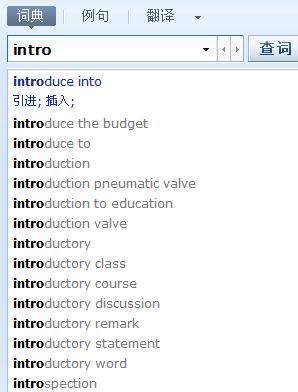
\includegraphics[scale=0.5]{img/ciba.eps}
  \caption{E-dictionary. All candidates starting with what the user input are listed.}
  \label{fig:e-dict}
\end{figure}

A E-dictionary typically contains hundreds of thousands words. It's very expensive
to performs a whole word search. Commercial software adopts complex approaches, including
caching, indexing etc to speed up this process.

Similar with e-dictionary, figure \ref{fig:word-completion} shows a popular
Internet search engine. When user input something, it provides a candidate
lists, with all items starting with what the user has entered. And these candidates
are shown in the order of popularity. The more people search, the
upper position it is in the list.

\begin{figure}[htbp]
  \centering
  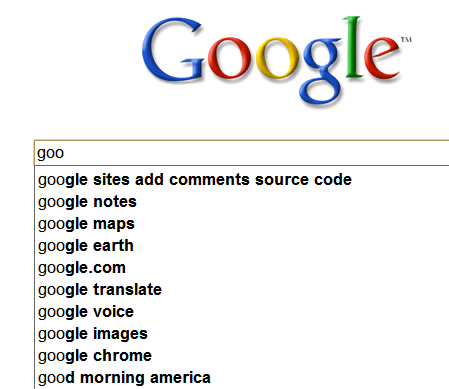
\includegraphics[scale=0.5]{img/adaptive-input.eps}
  \caption{A search engine. All candidates starting with what user input are listed.}
  \label{fig:word-completion}
\end{figure}

In both cases, the software provides a kind of word auto-completion mechanism.
In some modern IDEs, the editor can even help users to auto-complete program code.

Let's see how to implementation of the e-dictionary with trie or Patricia.
To simplify the problem, we assume the dictionary only supports English - English
information.

A dictionary stores key-value pairs, the keys are English
words or phrases, the values are the meaning described in English sentences.

We can store all the words and their meanings in a trie, but it isn't
space effective especially when there are huge amount of items. We'll use
Patricia to realize e-dictionary.

When user wants to look up word 'a', the dictionary does not only
return the meaning of 'a', but also provides a list of
candidate words, which all start with 'a', including 'abandon', 'about',
'accent', 'adam', ... Of course all these words are stored in the Patricia.

If there are too many candidates, one solution is only displaying the top 10
words, and the user can browse for more.

The following algorithm reuses the looking up defined for Patricia. When it
finds a node bound to a string which is the prefix of what we are looking for,
it expands all its children until getting $n$ candidates.

\begin{algorithmic}[1]
\Function{Look-Up}{$T, k, n$}
  \If{$T = $ NIL}
     \State \Return $\phi$
  \EndIf
  \State $prefix \gets$ NIL
  \Repeat
    \State $match \gets$ FALSE
    \For{$\forall (k_i, T_i) \in $ \Call{Children}{$T$}}
      \If{$k$ is prefix of $k_i$}
        \State \Return \Call{Expand}{$T_i, prefix, n$}
      \EndIf
      \If{$k_i$ is prefix of $k$}
        \State $match \gets$ TRUE
        \State $k \gets k - k_i$
        \State $T \gets T_i$
        \State $prefix \gets prefix + k_i$
        \State break
      \EndIf
    \EndFor
  \Until{$\lnot match$}
  \State \Return $\phi$
\EndFunction
\end{algorithmic}

Where function \textproc{Expand}($T, prefix, n$) picks $n$ sub trees, which
share the same prefix in $T$. It is realized as BFS (Bread-First-Search) traverse. Chapter search
explains BFS in detail.

\begin{algorithmic}[1]
\Function{Expand}{$T, prefix, n$}
  \State $R \gets \phi$
  \State $Q \gets \{(prefix, T)\}$
  \While{$|R| < n \land |Q| > 0$}
    \State $(k, T) \gets$ \Call{Pop}{$Q$}
    \If{\Call{Data}{$T$} $\neq$ NIL}
      \State $R \gets R \cup \{(k, $ \Call{Data}{$T$} $)\}$
    \EndIf
    \For{$\forall (k_i, T_i) \in$ \Call{Children}{$T$}}
      \State \Call{Push}{$Q, (k + k_i, T_i)$}
    \EndFor
  \EndWhile
\EndFunction
\end{algorithmic}

The following example Python program implements the e-dictionary application.
When testing if a string is prefix of another one, it uses the \texttt{find}
function provided in standard string library.

\lstset{language=Python}
\begin{lstlisting}
import string

def patricia_lookup(t, key, n):
    if t is None:
        return None
    prefix = ""
    while True:
        match = False
        for k, tr in t.children.items():
            if string.find(k, key) == 0: #is prefix of
                return expand(prefix+k, tr, n)
            if string.find(key, k) ==0:
                match = True
                key = key[len(k):]
                t = tr
                prefix += k
                break
        if not match:
            return None

def expand(prefix, t, n):
    res = []
    q = [(prefix, t)]
    while len(res)<n and len(q)>0:
        (s, p) = q.pop(0)
        if p.value is not None:
            res.append((s, p.value))
        for k, tr in p.children.items():
            q.append((s+k, tr))
    return res
\end{lstlisting}

This algorithm can also be implemented recursively, if the string we
are looking for is empty, we expand all children until getting $n$
candidates. Otherwise we recursively examine the children to
find one which has prefix equal to this string.

In programming environments supporting lazy evaluation. An intuitive
solution is to expand all candidates, and take the first $n$ on
demand. Denote the Patricia prefix tree in form $T = (v, C)$,
below function enumerates all items starts with key $k$.

\be
findAll(T, k) = \left \{
  \begin{array}
  {r@{\quad:\quad}l}
  enum(C) & k = \phi, v = \phi \\
  \{(\phi, v)\} \cup enum(C) & k = \phi, v \neq \phi \\
  find(C, k) & k \neq \phi
  \end{array}
\right.
\ee

The first two clauses deal with the edge cases the the key is empty.
All the children are enumerated except for those with empty values.
The last clause finds child matches $k$.

For non-empty children, $C = \{(k_1, T_1), (k_2, T_2), ..., (k_m, T_m)\}$,
denote the rest pairs except for the first one as $C'$.
The enumeration algorithm can be defined as below.

\be
enum(C) = \left \{
  \begin{array}
  {r@{\quad:\quad}l}
  \phi & C = \phi \\
  mapAppend(k_1, findAll(T_1, \phi)) \cup enum(C')
  \end{array}
\right.
\ee

Where $mapAppend(k, L) = \{(k + k_i, v_i)| (k_i, v_i) \in L\}$. It concatenate
the prefix $k$ in front of every key-value pair in list $L$.

Function $find(C, k)$ is defined as the following. For empty children, the
result is empty as well; Otherwise, it examines the first child $T_1$ which
is bound to string $k_1$. If $k_1$ is equal to $k$, it calls $mapAppend$ to
add prefix to the keys of all the children under $T_1$; If $k_1$ is prefix
of $k$, the algorithm recursively find all children start with $k - k_1$;
On the other hand, if $k$ is prefix of $k_1$, all children under $T_1$
are valid result. Otherwise, the algorithm by-pass the first child
and goes on find the rest children.

\be
find(C, k) = \left \{
  \begin{array}
  {r@{\quad:\quad}l}
  \phi & C = \phi \\
  mapAppend(k, findAll(T_1, \phi)) & k_1 = k \\
  mapAppend(k_1, findAll(T_1, k - k_1)) & k_1 \sqsubset k \\
  findAll(T_1, \phi) & k \sqsubset k_1 \\
  find(C', k) & otherwise
  \end{array}
\right.
\ee

Below example Haskell program implements the e-dictionary application
according to the above equations.

\lstset{language=Haskell}
\begin{lstlisting}
findAll :: Patricia a -> Key -> [(Key, a)]
findAll t [] =
    case value t of
      Nothing -> enum $ children t
      Just x  -> ("", x):(enum $ children t)
    where
      enum [] = []
      enum (p:ps) = (mapAppend (fst p) (findAll (snd p) [])) ++ (enum ps)
findAll t k = find' (children t) k where
    find' [] _ = []
    find' (p:ps) k
          | (fst p) == k
              = mapAppend k (findAll (snd p) [])
          | (fst p) `Data.List.isPrefixOf` k
              = mapAppend (fst p) (findAll (snd p) (k `diff` (fst p)))
          | k `Data.List.isPrefixOf` (fst p)
              = findAll (snd p) []
          | otherwise = find' ps k
    diff x y = drop (length y) x

mapAppend s lst = map (\p->(s++(fst p), snd p)) lst
\end{lstlisting}

In the lazy evaluation environment, the top $n$ candidates can be
gotten like $take(n, findAll(T, k))$. Appendix A has detailed definition
of $take$ function.

%=====================================
% T9
%=====================================

\subsection{T9 input method}
\index{T9}
\index{Textonym input method}

Most mobile phones around year 2000 are equipped with a key pad.
Users have quite different experience from PC when editing a short message
or email.
This is because the mobile-phone key pad, or so called ITU-T key pad has much fewer
keys than PC. Figure \ref{fig:itut-keypad} shows one example.

\begin{figure}[htbp]
  \centering
  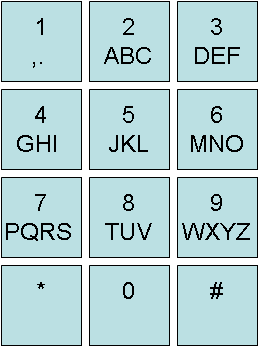
\includegraphics[scale=0.4]{img/itu-t.eps}
  \caption{an ITU-T keypad for mobile phone.}
  \label{fig:itut-keypad}
\end{figure}

There are typical two methods to input English word or phrases with ITU-T key pad.
For instance, if user wants to enter a word `home', He can press the key
in below sequence.

\begin{itemize}
\item Press key '4' twice to enter the letter 'h';
\item Press key '6' three times to enter the letter 'o';
\item Press key '6' twice to enter the letter 'm';
\item Press key '3' twice to enter the letter 'e';
\end{itemize}

Another much quicker way is to just press the following keys.

\begin{itemize}
\item Press key '4', '6', '6', '3', word `home' appears on top of the candidate list;
\item Press key '*' to change a candidate word, so word `good' appears;
\item Press key '*' again to change another candidate word, next word `gone' appears;
\item ...
\end{itemize}

Compare these two methods, we can see the second one is much easier for the end user.
The only overhead is to store a dictionary of candidate words.

Method 2 is called as `T9' input method, or predictive input method
\cite{wiki-t9}, \cite {wiki-predictive-text}. The abbreviation 'T9' stands
for 'textonym'. It start with 'T' with 9 characters. T9 input can also be
realized with trie or Patricia.

In order to provide candidate words to user, a dictionary must be prepared
in advance. Trie or Patricia can be used to store the dictionary. The
commercial T9 implementations typically use complex indexing dictionary in
both file system and cache. The realization shown here is for illustration
purpose only.

Firstly, we need define the T9 mapping, which maps from digit to candidate
characters.

\be
\begin{array}{ll}
M_{T9} = \{ & 2 \rightarrow abc, 3 \rightarrow def, 4 \rightarrow ghi, \\
           & 5 \rightarrow jkl, 6 \rightarrow mno, 7 \rightarrow pqrs, \\
           & 8 \rightarrow tuv, 9 \rightarrow wxyz \}
\end{array}
\ee

With this mapping, $M_{T9}[i]$ returns the corresponding characters for digit $i$.

Suppose user input digits $D = d_1d_2...d_n$, If $D$ isn't empty, denote the
rest digits except for $d_1$ as $D'$,
below pseudo code shows how to realize T9 with trie.

\begin{algorithmic}[1]
\Function{Look-Up-T9}{$T, D$}
  \State $Q \gets \{(\phi, D, T)\}$
  \State $R \gets \phi$
  \While{$Q \neq \phi$}
    \State $(prefix, D, T) \gets$ \Call{Pop}{$Q$}
    \For{each $c$ in $M_{T9}[d_1]$}
      \If{$c \in $ \Call{Children}{$T$}}
        \If{$D' = \phi$}
          \State $R \gets R \cup \{prefix + c\}$
        \Else
          \State \textproc{Push}($Q, (prefix + c, D', $ \Call{Children}{$t$}$[c])$)
        \EndIf
      \EndIf
    \EndFor
  \EndWhile
  \State \Return $R$
\EndFunction
\end{algorithmic}

Where $prefix + c$ means appending character $c$ to the end of string $prefix$.
Again, this algorithm performs BFS search with a queue $Q$. The queue is
initialized with a tuple $(prefix, D, T)$, containing empty prefix, the digit sequence to be
searched, and the trie. It keeps picking the tuple from the queue as far as
it isn't empty. Then get the candidate characters from the first digit to
be processed via the T9 map. For each character $c$, if there is a sub-tree
bound to it, we created a new tuple, update the prefix by appending $c$,
using the rest of digits to update $D$, and use that sub-tree. This new tuple
is pushed back to the queue for further searching. If all the digits are
processed, it means a candidate word is found. We put this word to the
result list $R$.

The following example program in Python implements this T9 search with trie.

\lstset{language=Python}
\begin{lstlisting}
T9MAP={'2':"abc", '3':"def", '4':"ghi", '5':"jkl", \
       '6':"mno", '7':"pqrs", '8':"tuv", '9':"wxyz"}

def trie_lookup_t9(t, key):
    if t is None or key == "":
        return None
    q = [("", key, t)]
    res = []
    while len(q)>0:
        (prefix, k, t) = q.pop(0)
        i=k[0]
        if not i in T9MAP:
            return None #invalid input
        for c in T9MAP[i]:
            if c in t.children:
                if k[1:]=="":
                    res.append((prefix+c, t.children[c].value))
                else:
                    q.append((prefix+c, k[1:], t.children[c]))
    return res
\end{lstlisting}

Because trie is not space effective, we can modify the above algorithm with
Patricia solution. As far as the queue isn't empty, the algorithm pops the
tuple. This time, we examine all the prefix-sub tree pairs. For every pair
$(k_i, T_i)$, we convert the alphabetic prefix $k_i$ back to digits sequence $D'$
by looking up the T9 map. If $D'$ exactly matches the digits of what user input,
we find a candidate word; otherwise if the digit sequence is prefix of what user inputs,
the program creates a new tuple, updates the prefix, the digits to be processed,
and the sub-tree. Then put the tuple back to the queue for further search.

\begin{algorithmic}[1]
\Function{Look-Up-T9}{$T, D$}
  \State $Q \gets \{(\phi, D, T)\}$
  \State $R \gets \phi$
  \While{$Q \neq \phi$}
    \State $(prefix, D, T) \gets$ \Call{Pop}{$Q$}
    \For{each $(k_i, T_i) \in $ \Call{Children}{$T$}}
      \State $D' \gets$ \Call{Convert-T9}{$k_i$}
      \If{$D' \sqsubset D$} \Comment{$D'$ is prefix of $D$}
        \If{$D' = D$}
          \State $R \gets R \cup \{prefix + k_i\}$
        \Else
          \State \textproc{Push}($Q, (prefix + k_i, D - D', T_i)$)
        \EndIf
      \EndIf
    \EndFor
  \EndWhile
  \State \Return $R$
\EndFunction
\end{algorithmic}

Function \textproc{Convert-T9}($K$) converts each character in $K$ back to digit.

\begin{algorithmic}[1]
\Function{Convert-T9}{$K$}
  \State $D \gets \phi$
  \For{each $c \in K$}
     \For{each $(d \rightarrow S) \in M_{T9}$}
       \If{$c \in S$}
         \State $D \gets D \cup \{d\}$
         \State break
       \EndIf
     \EndFor
  \EndFor
  \State \Return $D$
\EndFunction
\end{algorithmic}

The following example Python program implements the T9 input method with Patricia.

\lstset{language=Python}
\begin{lstlisting}
def patricia_lookup_t9(t, key):
    if t is None or key == "":
        return None
    q = [("", key, t)]
    res = []
    while len(q)>0:
        (prefix, key, t) = q.pop(0)
        for k, tr in t.children.items():
            digits = toT9(k)
            if string.find(key, digits)==0: #is prefix of
                if key == digits:
                    res.append((prefix+k, tr.value))
                else:
                    q.append((prefix+k, key[len(k):], tr))
    return res
\end{lstlisting}

T9 input method can also be realized recursively. Let's first define
the trie solution. The algorithm takes two arguments, a trie storing
all the candidate words, and a sequence of digits that is input by
the user. If the sequence is empty, the result is empty as well;
Otherwise, it looks up $C$ to find those children which are bound
to the first digit $d_1$ according to T9 map.

\be
findT9(T, D) = \left \{
  \begin{array}
  {r@{\quad:\quad}l}
  \{ \phi \} & D = \phi \\
  fold(f, \phi, lookupT9(d_1, C)) & otherwise
  \end{array}
\right.
\ee

Where folding is defined in Appendix A. Function $f$ takes two arguments,
an intermediate list of candidates which is initialized empty, and
a pair $(c, T')$, where $c$ is candidate character, to which sub tree $T'$
is bound. It append character $c$ to all the candidate words, and concatenate
this to the result list.

\be
f(L, (c, T')) = mapAppend(c, findT9(T', D')) \cup L
\ee

Note this $mapAppend$ function is a bit different from the previous one defined
in e-dictionary application. The first argument is a character, but not a string.

Function $lookupT9(k, C)$ checks all the possible characters mapped to digit $k$.
If the character is bound to some child in $C$, it is record as one candidate.

\be
lookupT9(d, C) =  fold(g, \phi, M_{T9}[k])
\ee

Where

\be
g(L, k) = \left \{
  \begin{array}
  {r@{\quad:\quad}l}
  L & find(C, k) = \phi \\
  \{(k, T')\} \cup L & find(C, k) = T'
  \end{array}
\right.
\ee

Below Haskell example program implements the T9 look up algorithm with trie.

\lstset{language=Haskell}
\begin{lstlisting}
mapT9 = [('2', "abc"), ('3', "def"), ('4', "ghi"), ('5', "jkl"),
         ('6', "mno"), ('7', "pqrs"), ('8', "tuv"), ('9', "wxyz")]

findT9 t [] = [("", value t)]
findT9 t (k:ks) = foldl f [] (lookupT9 k (children t))
    where
      f lst (c, tr) = (mapAppend' c (findT9 tr ks)) ++ lst

lookupT9 c children = case lookup c mapT9 of
        Nothing -> []
        Just s  -> foldl f [] s where
             f lst x = case lookup x children of
                 Nothing -> lst
                 Just t  -> (x, t):lst

mapAppend' x lst = map (\p->(x:(fst p), snd p)) lst
\end{lstlisting}

There are few modifications when change the realization from trie to Patricia.
Firstly, the sub-tree is bound to prefix string, but not a single character.

\be
findT9(T, D) = \left \{
  \begin{array}
  {r@{\quad:\quad}l}
  \{ \phi \} & D = \phi \\
  fold(f, \phi, findPrefixT9(D, C)) & otherwise
  \end{array}
\right.
\ee

The list for folding is given by calling function $findPrefixT9(D, C)$.
And $f$ is also modified to reflect this change. It appends the
candidate prefix $D'$ in front of every result output by the
recursive search, and then accumulates the words.

\be
f(L, (D', T')) = mapAppend(D', findT9(T', D - D')) \cup L
\ee

Function $findPrefixT9(D, C)$ examines all the children. For
every pair $(k_i, T_i)$, if converting $k_i$ back to digits
yields a prefix of $D$, then this pair is selected as a
candidate.

\be
findPrefixT9(D, C) = \{ (k_i, T_i) |(k_i, T_i) \in C, convertT9(k_i) \sqsubset D\}
\ee

Function $convertT9(k)$ converts every alphabetic character in $k$ back
to digits according to T9 map.

\be
convertT9(K) = \{ d | \forall c \in k, \exists (d \rightarrow S) \in M_{T9} \Rightarrow c \in S\}
\ee

The following example Haskell program implements the T9 input algorithm
with Patricia.

\begin{lstlisting}
findT9 t [] = [("", value t)]
findT9 t k = foldl f [] (findPrefixT9 k (children t))
    where
      f lst (s, tr) = (mapAppend s (findT9 tr (k `diff` s))) ++ lst
      diff x y = drop (length y) x

findPrefixT9 s lst = filter f lst where
    f (k, _) = (toT9 k) `Data.List.isPrefixOf` s

toT9 = map (\c -> head $ [ d |(d, s) <- mapT9, c `elem` s])
\end{lstlisting}

\begin{Exercise}
\begin{itemize}
\item For the T9 input, compare the results of the algorithms realized with trie and Patricia,
the sequences are different. Why does this happen? How to modify the algorithm so that they
output the candidates with the same sequence?
\end{itemize}
\end{Exercise}

% ================================================================
%                 Short summary
% ================================================================
\section{Summary}

In this chapter, we start from the integer base trie and Patricia. The
map data structure based on integer Patricia plays an important role
in Compiler implementation. Alphabetic trie and Patricia are
natural extensions. They can be used to manipulate text information.
As examples, predictive e-dictionary and T9 input method are
realized with trie or Patricia. Although these examples
are different from the real implementation in commercial software.
They show simple approaches to solve some problems.
Other important data structure, such as suffix tree, has close
relationship with them. Suffix tree is introduced in the next chapter.

\begin{thebibliography}{99}

\bibitem{CLRS}
Thomas H. Cormen, Charles E. Leiserson, Ronald L. Rivest and Clifford Stein.
``Introduction to Algorithms, Second Edition''. Problem 12-1. ISBN:0262032937. The MIT Press. 2001

\bibitem{okasaki-int-map}
Chris Okasaki and Andrew Gill. ``Fast Mergeable Integer
Maps''. Workshop on ML, September 1998, pages 77-86, http://www.cse.ogi.edu/~andy/pub/finite.htm

\bibitem{patricia-morrison}
D.R. Morrison, ``PATRICIA -- Practical Algorithm To Retrieve  Information Coded In Alphanumeric", Journal of the ACM, 15(4), October 1968, pages 514-534.

\bibitem{wiki-suffix-tree}
Suffix Tree, Wikipedia. http://en.wikipedia.org/wiki/Suffix\_tree

\bibitem{wiki-trie}
Trie, Wikipedia. http://en.wikipedia.org/wiki/Trie

\bibitem{wiki-t9}
T9 (predictive text), Wikipedia. http://en.wikipedia.org/wiki/T9\_(predictive\_text)

\bibitem{wiki-predictive-text}
Predictive text,
Wikipedia. http://en.wikipedia.org/wiki/Predictive\_text

\end{thebibliography}

\ifx\wholebook\relax\else
\end{document}
\fi
